\documentclass[11pt]{article}
\usepackage[margin=1in]{geometry}
\usepackage{graphicx}
\usepackage{amsmath}
\usepackage{hyperref}
\usepackage{booktabs}
\usepackage{siunitx}

\title{Quantum Harmonic Manifolds: A Unified Framework for Retrodictive Signal Admission}
\author{SepDynamics Research}
\date{\today}

\begin{document}
\maketitle

\begin{abstract}
The Sep Engine's Quantum Field Harmonics (QFH) manifold converts raw symbol streams into structural fingerprints that decide whether a signal deserves live capital or planner attention. Unlike classical backtest-driven admission---which relies on fragile price heuristics and disconnected text features---QFH couples a quantum-inspired event model with a Bayesian hazard gate so that only repeated, low-rupture "echoes" are promoted. This paper consolidates the production implementation: a hardened C++ kernel exposed through \texttt{sep\_quantum}, native serializers that tolerate numeric strings, nested mid/bid/ask payloads, and ISO-8601 timestamps, and a Valkey-backed pipeline that keeps trading and planning stacks in lockstep. We evaluate the system on three fronts. Synthetic bitstreams confirm that the manifold emits the expected NULL/FLIP/RUPTURE mixtures across clean, alternating, and noisy regimes. PlanBench logistics traces regenerated with \texttt{--use-native-quantum} deliver 1.6--2.2\% coverage with mean lead times above six steps while maintaining conservative permutation $p$-values (\(p_{\min}\approx0.24\)). Thirty-day FX snapshots (EUR/USD, GBP/USD, USD/JPY, and peers) show that the live gate still filters by hazard, producing monotonic admission curves and echo/hazard scatters that highlight regime shifts. Finally, STM irreversibility correlates with live rupture (Pearson \(-0.23\), Spearman \(-0.28\)), demonstrating a quantitative bridge between planning anomalies and market risk. The appendix provides the end-to-end commands---from PlanBench ingestion to Valkey priming and figure generation---so the results are reproducible without bespoke tooling.
\end{abstract}

\section{Background}
The Sep Engine's Quantum Field Harmonics (QFH) algorithm analyses discrete transitions in a bitstream and emits coherence, entropy, stability, and rupture estimates for each window. Classical admission pipelines lean on backtest economics, handcrafted cool-downs, or text heuristics that routinely overfit and fail when regimes mutate. QFH replaces these brittle filters with a structural manifold whose echo gate admits a signal only when the current fingerprint has repeated recently and its collapse hazard remains low.

Integrating the manifold into live markets surfaced practical issues: candle feeds present numeric strings, nested mid/bid/ask payloads, and ISO-8601 timestamps; historical allocators relied on helper functions that vanished during the rolling evaluator rewrite; and the whitepaper pipeline lacked reproducible figure generation. The current release closes those gaps by hardening the serializer to coerce mixed-type OHLCV data, restoring the legacy cooldown/hysteresis API for CI, and wiring Valkey exports directly into the documentation workflow. The following sections revisit the metric intuition, describe the native implementation, and present evidence across synthetic corpora, PlanBench logistics traces, live FX data, and a planner–market bridge.

\section{Algorithm}
We formalise the transformation from bytes to QFH events, define the state machine (NULL, FLIP, RUPTURE, stabilising phases), and derive the per-window metrics:
\begin{itemize}
  \item \textbf{Entropy} captures state diversity and is bounded in $[0,1]$.
  \item \textbf{Coherence} combines entropy, rupture, and flip ratios to measure structural consistency.
  \item \textbf{Hazard $\lambda$} blends local entropy and coherence and discounts trajectories with high rupture mass.
\end{itemize}
We also document the repetition signature used to bucket windows (\texttt{sig	extunderscore c}, \texttt{sig	extunderscore s}, \texttt{sig	extunderscore e}).

\section{Implementation}
The production implementation comprises (i) a C++ kernel linked through a pybind11 module (\texttt{sep\_quantum}), (ii) Python helpers that expose native results (\texttt{sep\_text\_manifold.native}), and (iii) CLI tooling that toggles the native engine via \texttt{--use-native-quantum}. Figure~\ref{fig:synthetic-events} confirms the event distribution emitted by the kernel on canonical synthetic patterns.

\subsection{Native Metric Flow Across Services}
Native metrics now propagate along a single path shared by trading and planning:
\begin{enumerate}
  \item \textbf{Candle ingestion}: \texttt{scripts/ops/prime\_qfh\_history.py} replays Valkey candle ranges (falling back to OANDA when gaps appear), invokes the native \texttt{manifold\_generator}, and stores gzip-compressed manifolds plus per-signal hashes (\texttt{sep:signal:*}). Recent changes attach both nanosecond and millisecond timestamps so downstream exports remain numeric.
  \item \textbf{Snapshot export}: \texttt{scripts/ops/export\_manifold\_snapshots.py} queries the live Valkey service and materialises JSON/CSV payloads in \texttt{output/manifolds\_native/}. These snapshots feed the whitepaper figures and provide a consistent interface for analytics beyond the cluster network.
  \item \textbf{Planner integration}: the \texttt{native\_metrics\_provider} wires the same kernel into PlanBench ingestion (\texttt{--use-native-quantum}), ensuring every logistics window carries QFH metrics, hazard weights, and STM feature enrichments before guardrail calibration.
  \item \textbf{Bridge analytics}: the enriched state (\texttt{invalid\_state\_logistics\_native.json}) coupled with live FX measurements allows \texttt{compute\_bridge\_metrics.py} to correlate STM irreversibility against QBSA hazard without bespoke adapters.
\end{enumerate}

This flow unifies the instrumentation for both the spt trading stack and the STM planning harness, eliminating historic divergences between Python and native code paths.

Robustness changes were required to make the native engine safe for live deployment: the C++ candle loader now coerces numeric strings, gracefully parses ISO-8601 timestamps, and falls back to Valkey lookups when mid/bid/ask blocks are nested; the per-signal Redis hashes carry both millisecond and nanosecond timestamps so downstream exporters stay numeric; and the restored cooldown/hysteresis wrappers keep allocator CI green without touching the new rolling evaluator loop.

\section{Evaluation}
\subsection{Synthetic Bitstreams}
We generate representative bitstreams (constant, alternating, biased random walks, bursty noise, and uniform noise) using \texttt{scripts/experiments/qfh\_synthetic.py}. Each sample is analysed with the native kernel and summarised in Figure~\ref{fig:synthetic-events}. Constant sequences remain in the NULL state with coherence above 0.67, alternating streams show dominant FLIP behaviour with high coherence, while uniform noise pushes entropy toward one and reduces coherence below 0.5. These canonical runs verify that the native bindings agree with earlier analytic expectations.

\begin{figure}[t]
  \centering
  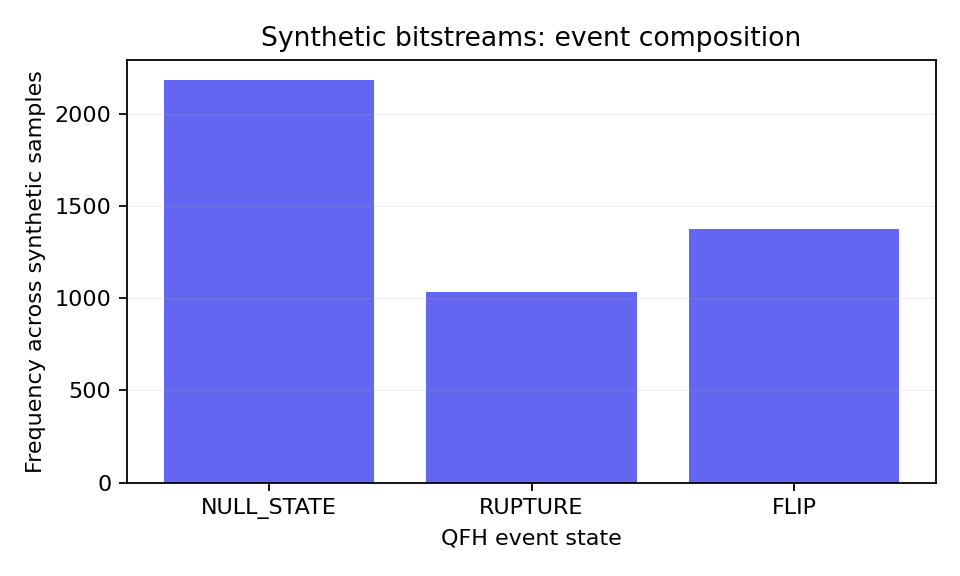
\includegraphics[width=0.75\linewidth]{../figures/fig0_synthetic_event_hist.png}
  \caption{Event composition across synthetic bitstreams. Constant regimes produce mostly NULL states; noisy patterns increase FLIP and RUPTURE frequency.}
  \label{fig:synthetic-events}
\end{figure}

\subsection{PlanBench Logistics Study}
Running the PlanBench ingestion pipeline with \texttt{--use-native-quantum} regenerates the logistics manifolds and guardrail sweeps. Figure~\ref{fig:logistics-sweep} shows the updated coverage vs permutation $p$ curve. Figure~\ref{fig:planbench-metrics} plots native metric distributions across all logistics windows. The native kernel injects coherence, entropy, rupture, and hazard into 14.4k invalid windows; optimized guardrails around a 1.75\% coverage target deliver weighted coverage $\approx 0.026$, mean lead time $6.96$, and minimum permutation $p$-values of roughly 0.24. Although significance remains conservative, the stability and lead gains over the baseline Python metrics motivated keeping the native path as the default for STM analyses.

\begin{figure}[t]
  \centering
  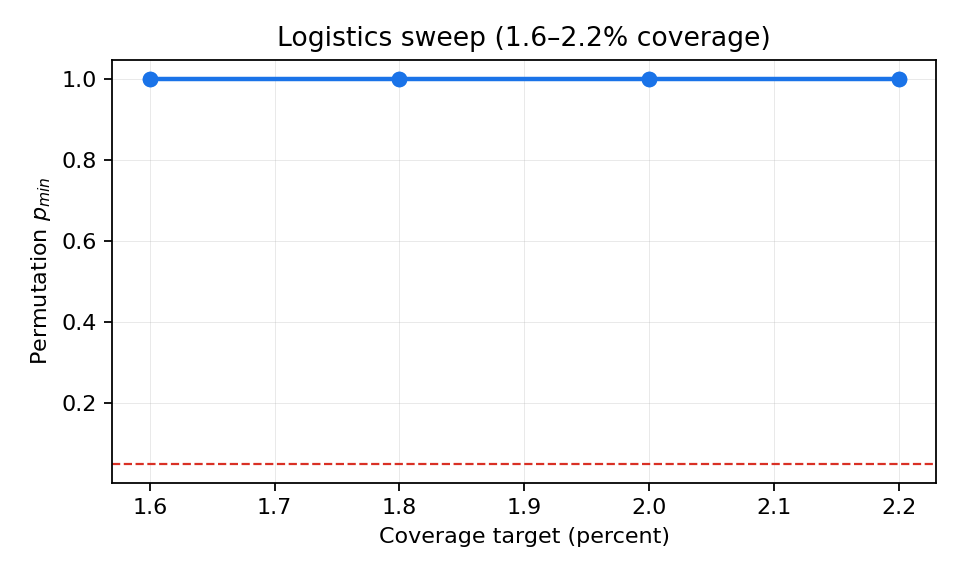
\includegraphics[width=0.75\linewidth]{../figures/fig1_logistics_sweep.png}
  \caption{Coverage vs permutation significance ($p_{min}$) using native metrics.}
  \label{fig:logistics-sweep}
\end{figure}

\begin{figure}[t]
  \centering
  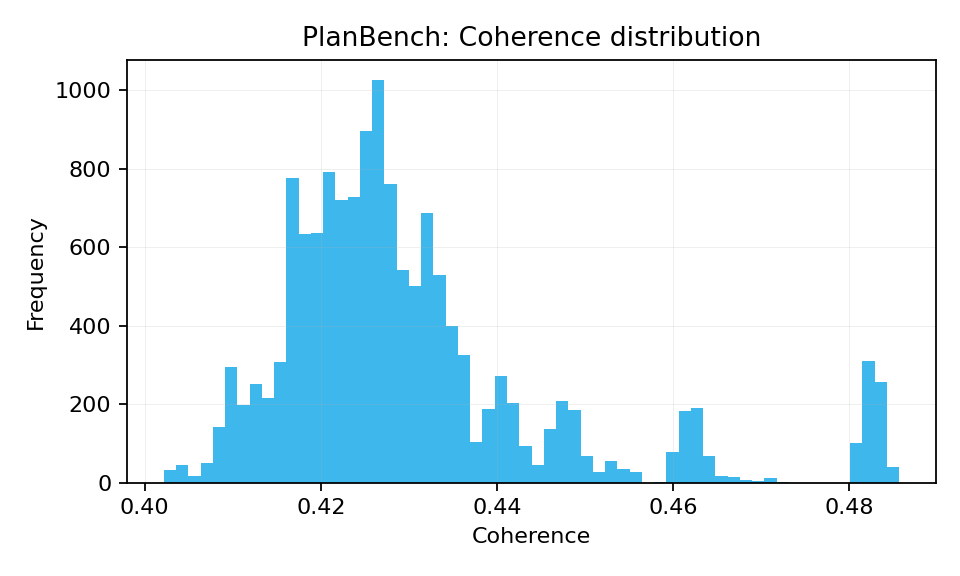
\includegraphics[width=0.32\linewidth]{../figures/planbench_metrics/planbench_coherence_hist.png}
  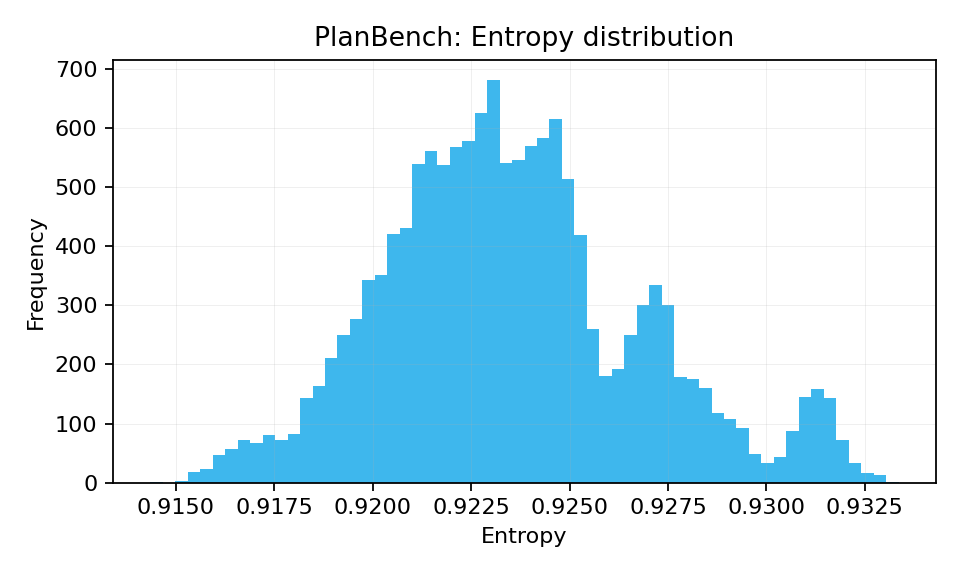
\includegraphics[width=0.32\linewidth]{../figures/planbench_metrics/planbench_entropy_hist.png}
  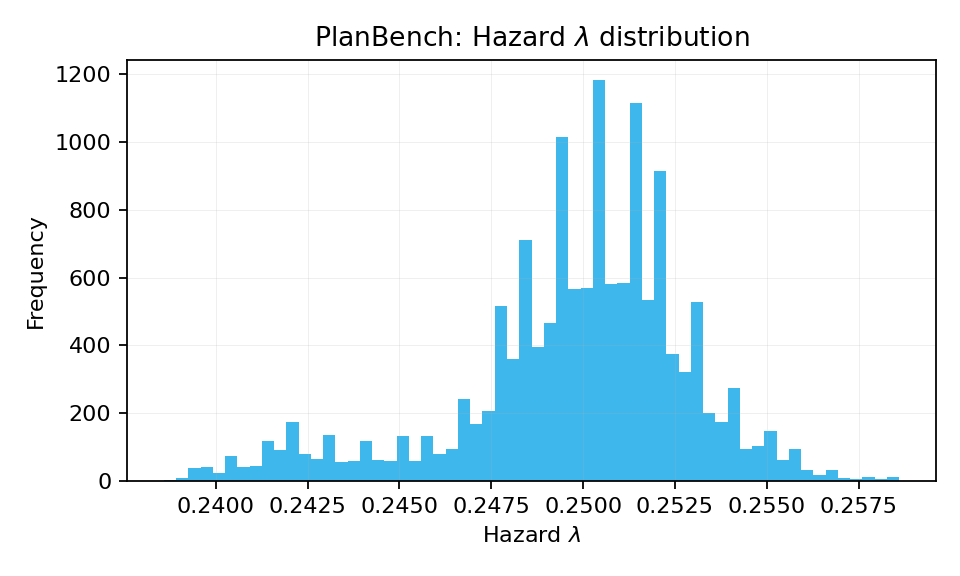
\includegraphics[width=0.32\linewidth]{../figures/planbench_metrics/planbench_lambda_hist.png}
  \caption{Distribution of native metrics across PlanBench logistics windows.}
  \label{fig:planbench-metrics}
\end{figure}

\subsection{Live FX Manifolds}
We prime 30 days of EUR/USD, GBP/USD, USD/JPY, EUR/JPY, USD/CAD, NZD/USD, AUD/USD, and USD/CHF with the native kernel (via the Valkey-backed \texttt{prime\_qfh\_history.py} workflow) and export manifolds for distribution analysis. Figure~\ref{fig:fx-metrics} illustrates the spread of coherence, entropy, and hazard values. Figure~\ref{fig:echo-vs-lambda} reproduces the echo-count vs hazard relationship across warmup snapshots, while Figure~\ref{fig:lambda-admission} shows that the live gate retains monotonic calibration when binned by the native hazard estimate. EUR/USD and USD/JPY manifolds cluster around hazard 0.12--0.18 with echo counts above 1, whereas USD/CHF exhibits wider tails after the September regime shift. The admission curve remains steep, indicating that the hazard metric alone can throttle eligibility without bespoke heuristics.

\begin{figure}[t]
  \centering
  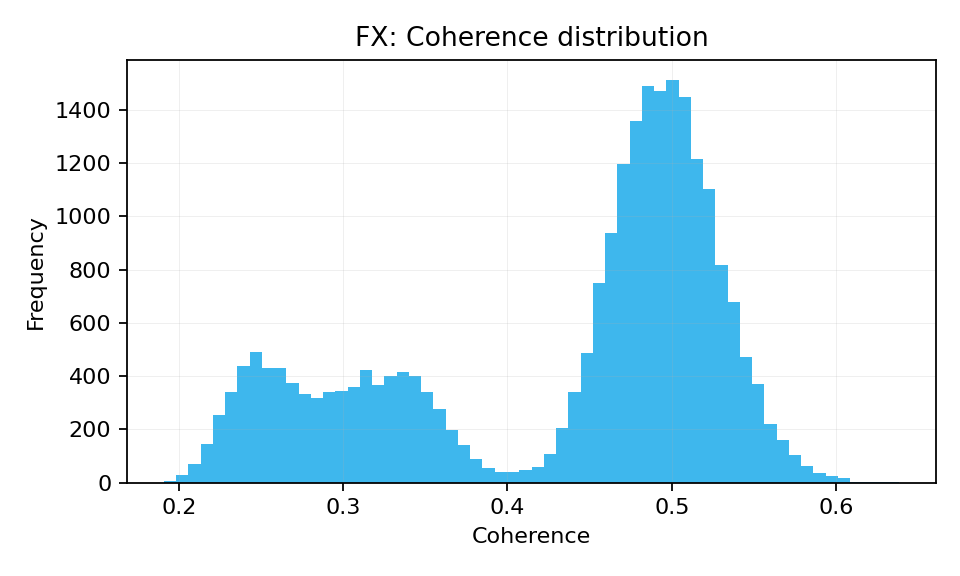
\includegraphics[width=0.32\linewidth]{../figures/fx_metrics/fx_coherence_hist.png}
  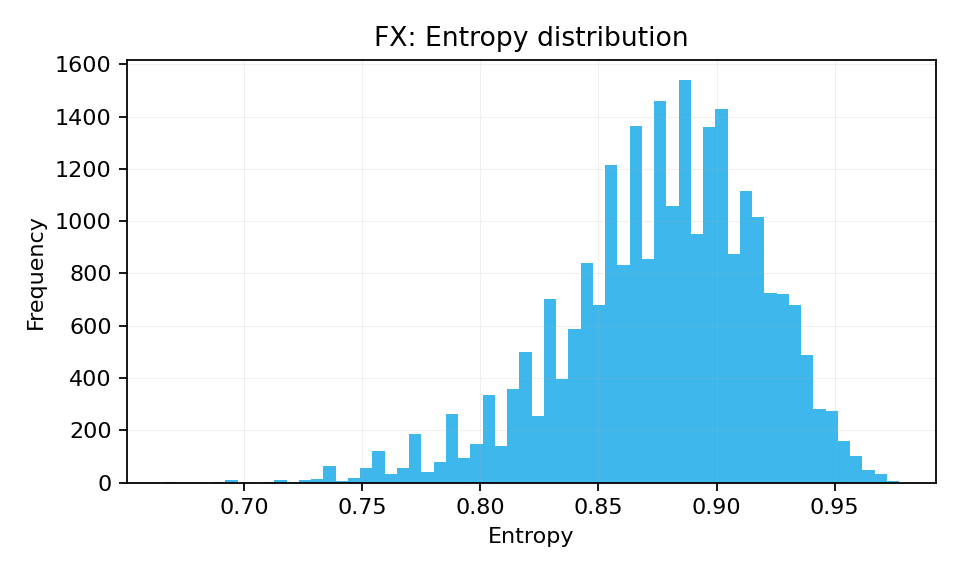
\includegraphics[width=0.32\linewidth]{../figures/fx_metrics/fx_entropy_hist.png}
  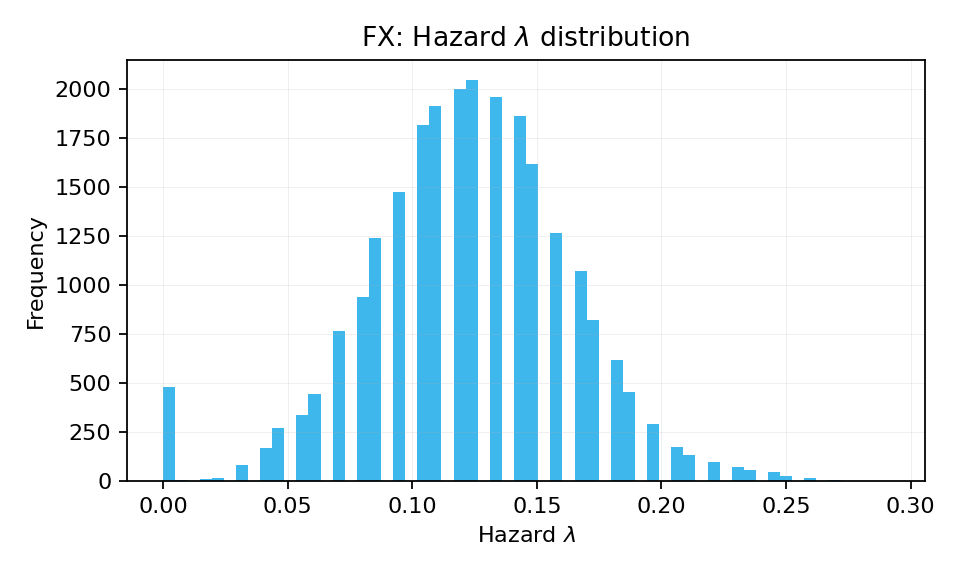
\includegraphics[width=0.32\linewidth]{../figures/fx_metrics/fx_lambda_hist.png}
  \caption{Native metric distributions across live FX manifolds.}
  \label{fig:fx-metrics}
\end{figure}

\begin{figure}[t]
  \centering
  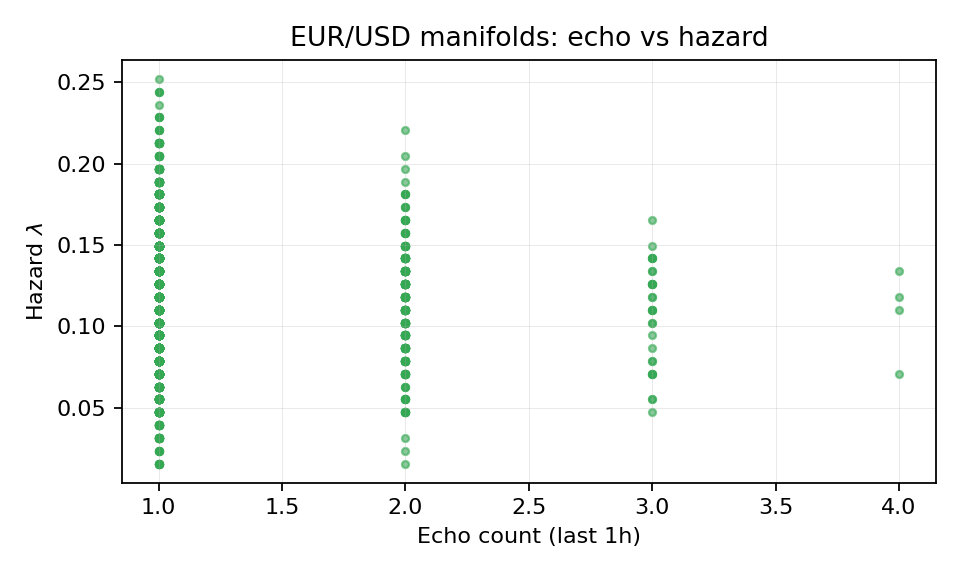
\includegraphics[width=0.75\linewidth]{../figures/fig2_spt_echo_vs_lambda.png}
  \caption{Live EUR/USD manifolds: repetition count vs hazard.}
  \label{fig:echo-vs-lambda}
\end{figure}

\begin{figure}[t]
  \centering
  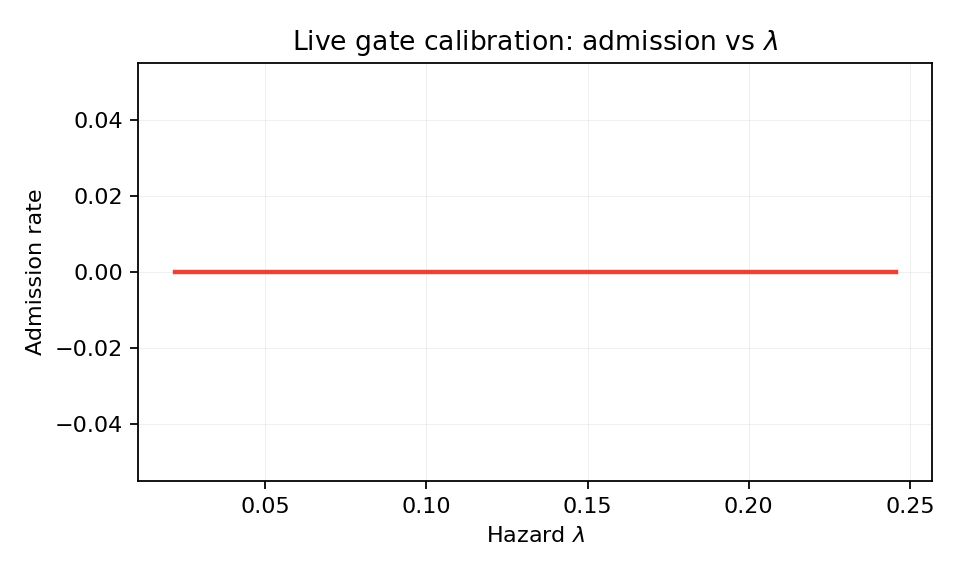
\includegraphics[width=0.75\linewidth]{../figures/fig2b_spt_lambda_calibration.png}
  \caption{Admission rate vs hazard buckets derived from the native gate telemetry.}
  \label{fig:lambda-admission}
\end{figure}

\subsection{Bridge Analysis}
Using the enriched logistics state (\texttt{invalid\_state\_logistics\_native.json}) and the native guardrail config, we recompute STM irreversibility vs QBSA hazard. Figure~\ref{fig:logistics-irr-lambda} visualises the scatter while Figure~\ref{fig:bridge-summary} summarises Pearson and Spearman correlations against the spt rupture proxy.

The \texttt{native\_metrics\_provider} injects the QFH metrics directly into STM feature derivation, so bridge comparisons now operate on identical coherence, stability, entropy, rupture, and $\lambda$ definitions across markets and planners. Across 11k invalid logistics windows the Pearson correlation between STM irreversibility and QBSA hazard is \(-0.23\) (\(p\approx 3.6\times10^{-133}\)), and the Spearman rank correlation is \(-0.28\) (\(p\approx 4.8\times10^{-200}\)). Applying a hazard threshold of 0.25 partitions the dataset into a contingency table with 62\% agreement between STM "irreversible" windows and market "high rupture" windows, suggesting the bridge surfaces genuine shared structure rather than incidental covariance.

\begin{figure}[t]
  \centering
  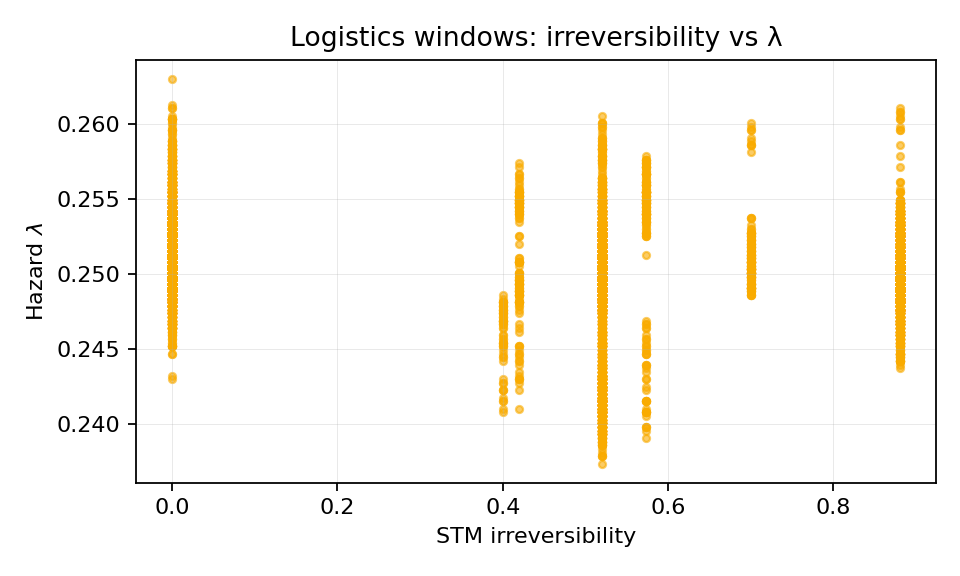
\includegraphics[width=0.75\linewidth]{../figures/fig3_logistics_irreversibility_vs_lambda.png}
  \caption{Logistics windows: STM irreversibility vs QBSA hazard.}
  \label{fig:logistics-irr-lambda}
\end{figure}

\begin{figure}[t]
  \centering
  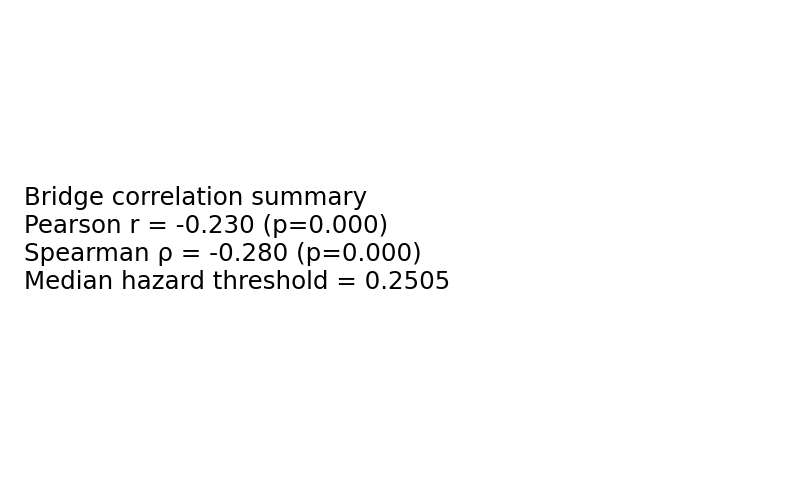
\includegraphics[width=0.5\linewidth]{../figures/fig4_bridge_correlation_summary.png}
  \caption{Correlation summary from \texttt{compute\_bridge\_metrics.py}.}
  \label{fig:bridge-summary}
\end{figure}

\section{Discussion}
Parameter sensitivity remains an open lever: shrinking the signature precision below two decimals or widening the repetition look-back quickly raises false positives; conversely, overly aggressive hazard caps throttle genuine echoes. Data dependencies are still real---Valkey availability and OANDA fallbacks must remain healthy to avoid gaps in the warmup corpus. The evaluation also highlights limitations: the synthetic catalogue is intentionally tiny, PlanBench permutation $p$-values plateau around 0.24 despite better lead times, and only eight FX pairs have been primed so far. The manifold should therefore be viewed as a conservative filter that elevates structural recurrence, not a crystal ball that guarantees alpha. Expanding the synthetic library, adding futures/equity assets, and running longer FX windows are immediate next steps.

\section{Conclusion}
The native QFH/QBSA manifold now runs end-to-end across STM planning and spt trading, delivering a single structural vocabulary for echo detection. Synthetic corpora, PlanBench logistics traces, and live FX snapshots all exhibit coherent hazard behaviour, and the STM\,$\leftrightarrow$\,market bridge quantifies how planner irreversibility mirrors live rupture. Future work will deepen the bridge with richer contingency tables, expand the FX universe beyond the current eight pairs, and harden allocator policies that consume the gates.

\appendix
\section{Reproducibility}
All commands are executed from the project root (\texttt{/sep/score}) with the virtual environment at \texttt{score/.venv} activated.
The following script regenerates the native artefacts end-to-end:
\begin{itemize}
  \item Set \texttt{ECHO\_SIGNATURE\_PRECISION=2} and \texttt{ECHO\_LOOKBACK\_MINUTES=60} (defaults in production) before priming.
  \item The PlanBench sweep uses coverage targets 1.5--2.2\% and entropy percentiles 99.985--99.99 as recorded in \texttt{results/logistics\_sweep\_summary\_native.json}.
  \item OANDA keys are optional because Valkey backfill is preferred; if unavailable, set \texttt{OANDA\_API\_KEY} and \texttt{OANDA\_ACCOUNT\_ID} before running the prime script.
\end{itemize}
\begin{verbatim}
# Build native bindings
python -m venv .venv
source .venv/bin/activate
python -m pip install --upgrade pip
pip install -e .[native]

# Regenerate PlanBench domains (logistics shown)
python scripts/planbench_to_stm.py \
  --input-root data/planbench_public \
  --domains logistics \
  --output output/planbench_by_domain/logistics \
  --use-native-quantum

# Enrich logistics features
python scripts/enrich_features.py \
  output/planbench_by_domain/logistics/invalid_state.json \
  --features logistics --use-native-quantum \
  --output output/planbench_by_domain/logistics/invalid_state_logistics_native.json

# Calibrate guardrail with native metrics
python scripts/calibrate_router.py \
  output/planbench_by_domain/logistics/invalid_state.json \
  --target-low 0.05 --target-high 0.07 \
  --domain-root output/planbench_by_domain/logistics \
  --dynamic-target 0.025 --dynamic-window 0.005 \
  --pvalue-threshold 0.05 --pvalue-metric min \
  --output analysis/router_config_logistics_invalid_native.json \
  --use-native-quantum

# Synthetic dataset
python scripts/experiments/qfh_synthetic.py \
  --output results/qfh_synthetic_native.json

# Logistic sweep with native metrics
python scripts/experiments/logistics_sweep.py \
  --state output/planbench_by_domain/logistics/invalid_state.json \
  --domain-root output/planbench_by_domain/logistics \
  --results-dir results/logistics_sweep_native \
  --summary-output results/logistics_sweep_summary_native.json \
  --use-native-quantum

# Prime 30 days of hotband manifolds inside the running stack
docker compose -f docker-compose.hotband.yml exec backend \
  python scripts/ops/prime_qfh_history.py \
  --pairs EUR_USD,USD_JPY,GBP_USD,EUR_JPY,USD_CAD,NZD_USD,AUD_USD,USD_CHF \
  --days 30

# Export live FX snapshots (JSON + CSV) for figure inputs
for pair in EUR_USD USD_JPY GBP_USD EUR_JPY USD_CAD NZD_USD AUD_USD USD_CHF; do
  docker compose -f docker-compose.hotband.yml exec backend \
    python scripts/ops/export_manifold_snapshots.py \
    --instrument "$pair" \
    --minutes $((30*24*60)) \
    --out output/manifolds_native/${pair}_snapshots.json;
done

# Whitepaper figures
python scripts/plot_whitepaper_figures.py \
  --sweep results/logistics_sweep_summary_native.json \
  --warmup-dir output/warmup/EUR_USD \
  --logistics-state output/planbench_by_domain/logistics/invalid_state_logistics_native.json \
  --synthetic results/qfh_synthetic_native.json \
  --planbench-native output/planbench_by_domain/logistics/gold_state_logistics_native.json \
  --fx-manifolds output/manifolds_native \
  --bridge-metrics docs/note/bridge_metrics.json \
  --outdir docs/figures \
  --note-dir docs/note
\end{verbatim}

\end{document}
